\documentclass[12pt]{extarticle}
%Some packages I commonly use.
\usepackage[english]{babel}
\usepackage{graphicx}
\usepackage{framed}
\usepackage[normalem]{ulem}
\usepackage{amsmath}
\usepackage{amsthm}
\usepackage{amssymb}
\usepackage{amsfonts}
\usepackage{enumerate}
\usepackage[utf8]{inputenc}
\usepackage[top=1 in,bottom=1in, left=1 in, right=1 in]{geometry}

%A bunch of definitions that make my life easier
\newcommand{\matlab}{{\sc Matlab} }
\newcommand{\cvec}[1]{{\mathbf #1}}
\newcommand{\rvec}[1]{\vec{\mathbf #1}}
\newcommand{\ihat}{\hat{\textbf{\i}}}
\newcommand{\jhat}{\hat{\textbf{\j}}}
\newcommand{\khat}{\hat{\textbf{k}}}
\newcommand{\minor}{{\rm minor}}
\newcommand{\trace}{{\rm trace}}
\newcommand{\spn}{{\rm Span}}
\newcommand{\rem}{{\rm rem}}
\newcommand{\ran}{{\rm range}}
\newcommand{\range}{{\rm range}}
\newcommand{\mdiv}{{\rm div}}
\newcommand{\proj}{{\rm proj}}
\newcommand{\R}{\mathbb{R}}
\newcommand{\N}{\mathbb{N}}
\newcommand{\Q}{\mathbb{Q}}
\newcommand{\Z}{\mathbb{Z}}
\newcommand{\<}{\langle}
\renewcommand{\>}{\rangle}
\renewcommand{\emptyset}{\varnothing}
\newcommand{\attn}[1]{\textbf{#1}}
\theoremstyle{definition}
\newtheorem{theorem}{Theorem}
\newtheorem{corollary}{Corollary}
\newtheorem*{definition}{Definition}
\newtheorem*{example}{Example}
\newtheorem*{note}{Note}
\newtheorem{exercise}{Exercise}
\newcommand{\bproof}{\bigskip {\bf Proof. }}
\newcommand{\eproof}{\hfill\qedsymbol}
\newcommand{\Disp}{\displaystyle}
\newcommand{\qe}{\hfill\(\bigtriangledown\)}
\setlength{\columnseprule}{1 pt}

\title{IDP Project Proposal}
\date{6 March, 2020}

\begin{document}

\maketitle

\section{Project idea}
Implementation of LDPC (Low density Parity Check Codes) in Python. 
The purpose of this project is to design and implement the LDPC coding and decoding and to compare the efficiency with other channel coding and decoding techniques. \\

\textbf{Type of Project:} Software based \newline

\textbf{Mentor/Instructor:} Dr. Shashank Vatedka

\section{Team Details}
\begin{itemize}
    \item Shaik Mastan Vali - EE18BTECH11039
    \item J. Prabhath Lakshminarayana - EE18BTECH11021
    \item K. Srikanth - EE18BTECH11023
\end{itemize}

\section{Introduction}
In information theory, a low-density parity-check (LDPC) code is a linear error correcting code, a method of transmitting a message over a noisy transmission channel. An LDPC is constructed using a sparse Tanner graph(a sub-class of bipartite graph). LDPC codes are capacity-approaching codes, which means that practical constructions exist that allow the noise threshold to be close to the Shannon limit. \\ \\
Impractical to implement when first developed by Gallager in 1963, LDPC codes were forgotten until his work was rediscovered in 1996. However, the advances in low-density parity-check codes have seen them surpass turbo codes in terms of error floor and performance in the higher code rate range, leaving turbo codes better suited for the lower code rates only. \\

\section{Brief Explanation}
LDPC codes functionally are defined by a sparse parity-check matrix \textbf{H}. In this graph, n variable nodes in the top of the graph are connected to $(n-k)$ constraint nodes in the bottom of the graph.

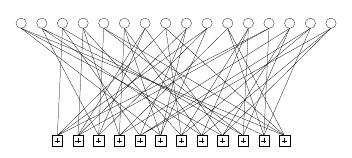
\includegraphics[scale = 2]{1.jpg} \newline
A low-density parity-check matrix and the corresponding graph of a $rate = \frac{1}{4}$ low-density parity-check code with blocklength N = 16, and
M = 12 constraints. Each white circle represents a transmitted bit.
Each bit participates in j = 3 constraints, represented by squares. Each constraint forces the sum of the k = 4 bits to which it is connected to be even.\\ \\
The generator matrix \textbf{G} can be constructed such that \textbf{G} is orthogonal to \textbf{H}. 
\begin{equation} \Rightarrow \textbf{G}\textbf{H}^T = 0 \end{equation}

As with other codes, the maximum likelihood decoding of an LDPC code on the binary symmetric channel is an \textbf{NP-complete problem}. However, sub-optimal techniques based on iterative \textbf{belief propagation} decoding give excellent results and can be practically implemented. 

The sub-optimal decoding techniques view each parity check that makes up the LDPC as an independent single parity check (SPC) code. Each SPC code is decoded separately using soft-in-soft-out (SISO) techniques. The soft decision information from each SISO decoding is cross-checked and updated with other redundant SPC decodings of the same information bit. Each SPC code is then decoded again using the updated soft decision information. This process is iterated until a valid code word is achieved or decoding is exhausted. This type of decoding is often referred to as sum-product decoding. \\

\textbf{Deliverable: }Implementation of the above mentioned algorithm and comparing the accuracy and time complexity with other channel coding techniques of the same type. \\

\textbf{Source: }Information Theory, Inference and Learning Algorithms by David J.C. McKay



\end{document}
